\documentclass{article}
\usepackage[utf8]{inputenc}

\title{\textbf{Project Abstract} \\ jetPR - A mobile robot with onboard GPU accelerated SLAM}
\author{Aswin Gururaj .P, Naven S.R, S. Srikrishna }
\date{}

\usepackage{natbib}
\usepackage{graphicx}

\begin{document}

\maketitle

\section{Introduction}
In recent times the advent of various technologies has made the comfort and leisure during life a strong priority. With the advent of robotics, this is ever more prevalent as the physical tasks to be done by humans are reduced. So to go with this trend we suggest the development of a mobile robot for indoor use using commercially available hardware and fully open-source software. Hence, the idea of jetPR (jetson Personal Robot) was conceived.

\begin{figure}[h!]
\centering
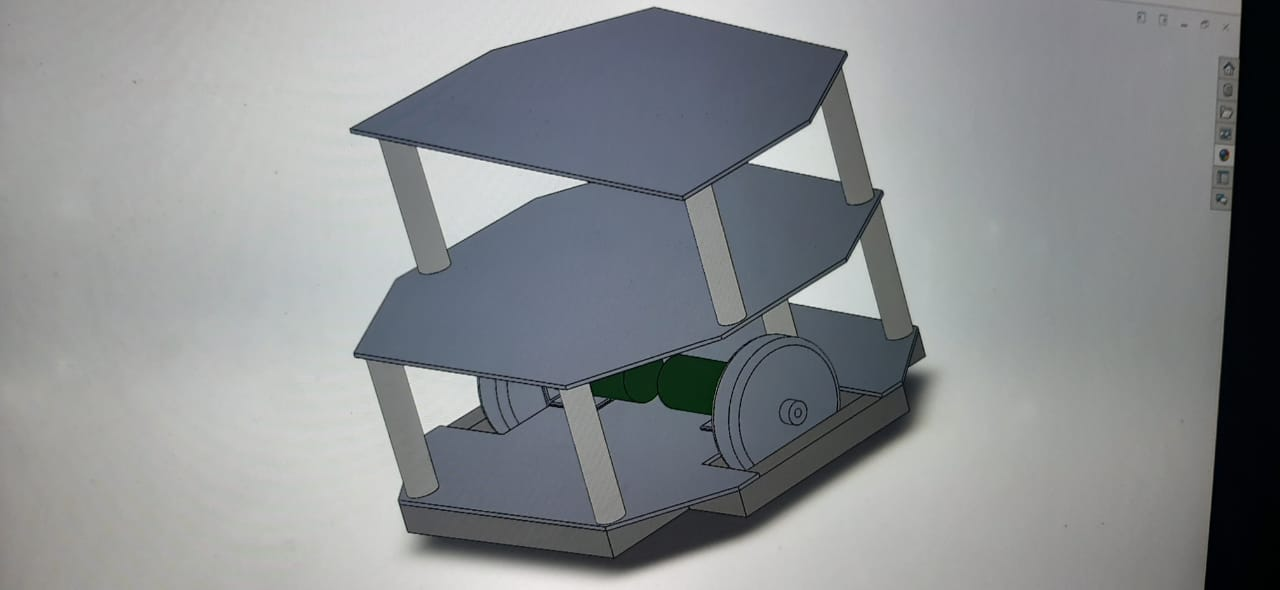
\includegraphics[scale=0.17]{robotdesign.jpeg}
\caption{Design of robot}
\label{fig:universe}
\end{figure}

The robot would be a differential drive robot with small dimensions ideal for indoor use and a stackable structure for future development. It would contain an Intel realsense RGB-D camera for mapping the area and localization in the map. It would contain encoded motors for odometry to allow the robot to estimate it own position. All the computation of the robot would occur on the onboard Nvidia Jetson Nano which is a powerful platform but in a small footprint to allow development of robotics and AI applications. The main objective however is to learn and implement an hardware accelerated SLAM (Simultaneous Localization and Mapping Algorithm) on the robot by using the onboard GPU for acceleration. Once this is done we plan to implement navigation algorithms which will allow the robot to move in a path planned by itself given destination in a dynamically changing environment.

\section{Design}
The robot was built with T Slot Aluminium Extrusion Frame with an Aluminium Alloy Base Plate held together with Steel L clamps. This design has been found to be very robust and is capable of high amount of stress. Also heavy duty wheels made of Silicone Rubber have been used as wheels and 2 caster wheels have been used. The motors used are high torque 300RPM DC geared motors with integrated encoders.

\section{Power Supply}
The power supply of choice was Li-Ion batteries because of their high energy desity and form factor. A 4S3P battery was chosen because of the capacity and voltage requirements of the robot. 2 Buck converters are used in the power circuit to convert the ~14.8V (4 3.7V Li-Ion cells) to 12V and 5V respectively. The 12V is to be supplied to the motors and the 5V to be supplied to the control and processing hardware.

\section{Control Hardware}
For controlling the DC motors we are using a dual channel H-Bridge DC motor driver which is capable of choosing direction of motor rotation and also is able to control the speed of the motor with external signals. The external signals are produced by an Arduino Mega containing an ATMega 2560 micro-controller which has to perform speed of motor measurement from the integrated encoders and provide the required PWM signal to the motor driver which powers the motor. The control hardware gets input from the processing hardware.

\section{Sensors and Camera}
We are planning to use HC SR04 ulrasonic sensors for low level obstacle detection and to use the Intel realsense D415 RGB-D camera for our mapping applications and for localization. The ultrasonic sensors are able to detect objects with 3mm accuracy for a range of 2m and the camera is used for creating a pointcloud data of the surrounding which is required for SLAM(Simultaneous Localization and Mapping). The camera is able to produce depth output at 1280x720 pixels at 90 frames per second.

\section{Processing Hardware}
We are using the NVIDIA jetson Nano embedded board for our processing applications. It runs embedded Linux which is based on Ubuntu 18.04 called Jetpack. Our objective is to run Robot Operating System on this framework. This allows us to access many open source programs for various applications of the robot allowing us to focus on ur problem statement. The jetson Nano has 128 CUDA cores for General Purpose GPU compute purposes and an ARM A57 running at 1.6GHz chip as a processor, This allows us to perform various compute operations.

\section{Odometry}
Odometry is the process of estimating the distance travelled and path travelled by the robot
by mounting sensors on the shaft of the actuator.  This can be used in the case of differential drive robots such as jetPR to estimate the x,y, yaw of the robot when it moves on a flat horizontal plane. However, this requires the assumption of pure rolling and no noise.  So we adopt a probabilistic version of this model.

\section{SLAM}
Simultaneous Localization and Mapping is a process where a robot can map the environment and also uses features of the environment to determine its pose in it. It can be achieved Extended Kalman filter and Particle filter. The data from the wheel odometry of the robot and the data obtained from the RGB-D intel realsense sensor are the input data to this method. It allows the robot to robustly estimate its pose with a probabilistic model rather than a deterministic model. Our objective is to perform this by using GPU accelerated hardware of the jetson nano.

\section{Navigation}
The process of moving the robot autonomously from place to place in a known map is called navigation. The robot is equipped to navigate in the environment using a map of the environment and the wheel odometry data. When given a goal point, the robot plans a global path based on the map which it has. It also plans a local path based on the immediate sensor data it receives from the RGB-D sensor. This ensures that the robot can perform static and dynamic obstacle avoidance. It uses A* search algorithm for global path planning and DWA planner for local motion planning. To interface all this, ROS provides a package called the navigation stack, which makes the development of a mobile robot a much faster job. The navigation stack requires parameters which have to be tuned based on the attributes of the robot currently working on, and once the parameters are set, the robot is ready to navigate in a map.

\bibliographystyle{plain}
\end{document}
